%図の挿入,箇条書きなどの材料です
\if0
%pdf挿入
\begin{figure}[h]
	\begin{center}
	\includegraphics[width=15cm, bb=0 0 1000 540, clip]{nfs.pdf}
	\caption{NFSを用いたファイル共有}
	\label{fig;db1}
	\end{center}
\end{figure}

%黒丸記号箇条書き
\begin{itemize}
\item 図書館の各テーブルに音を集音するマイク,,
\end{itemize}

%見出し付き箇条書き
\begin{description}
	\item[(1)図書館に設置する Raspbery PI (音声情報の入出力を行う Raspbery PI )]\mbox{}\\
 Raspbery PI (ラズベリーパイ)を
\end{description}

%番号付き箇条書き
\begin{enumerate}
 \item 騒音のレベルを測るための集音装置と,
\end{enumerate}

%表
\begin{tabular}{|l|c|}
\hline
 Raspberry Pi & 1台 \\ \hline
 無線LAN子機 & 1個 \\ \hline
\end{tabular}
\fi


%本文
%目次付けるには2回コンパイルが必要です
\documentclass[a4j,titlepage]{jarticle}
\usepackage[dvipdf]{graphicx}
\usepackage{url}
\usepackage{here}
\usepackage{ascmac}
\usepackage{amsmath}
\usepackage{color}
\title{
\vspace{30mm}
{\bf 図書館環境改善システム}
\\
\vspace{5mm}
SIZKANIC\\
\vspace{5mm}
{\bf 内部設計書}\\
\vspace{30mm}
{\bf 第0.0版}
\vspace{60mm}
}
\author{
{\large 株式会社 Divea}
}

\begin{document}
\maketitle

\tableofcontents

\newpage

\section{開発環境}
SIZKANICを開発するにあたり,次の開発環境を利用する.

\begin{itemize}
\item プログラミング言語 Python,JavaScript,CGI,html,PHP

\item 設計書作成ソフト TeXworks,Microsoft PowerPoint

\item データベース管理システム MySQL

\item バージョン管理 git,Dropbox

\end{itemize}
\section{動作環境}
SIZKANICの動作環境は,次の通りである.\\
\if0
※現在レンタルしているサーバ
\begin{description}
 \item[OS         :] Linux(CentoOS6 x86\_64)
 \item[Webサーバ      :] Apache
 \item[CPU       :] 仮想2Core
 \item[メモリ        :] 1GB
 \item[ハードディスク   :] 100GB
\end{description}

※KUT LMSのテンプレと同様のメモリ(4GB)のサーバをレンタルした場合
\fi
\begin{description}
 \item[OS         :] Linux(CentoOS6 x86\_64)
 \item[Webサーバ    :] Apache
 \item[CPU       :] 仮想4Core
 \item[メモリ       :] 4GB
 \item[ハードディスク   :] 400GB
\end{description}
\section{モジュール(メソッド)仕様}
\subsection{モジュール(メソッド)構成}
騒音情報表示端末,管理用端末は,Webブラウザを用いて表示をするため,騒音情報表示及びシステム管理に関するモジュールは騒音情報サーバに集約される(図X).

警告音出力端末,音取得端末は Raspbery PI が行うため,警告及び音取得に関するモジュールは Raspbery PI に集約される(図N).

騒音情報サーバは,次のモジュールで構成される.
  \begin{itembox}[l]{騒音情報表示に関するモジュール}
\begin{itemize}
\item ユーザ画面表示モジュール
\item dB値取得モジュール
\item データ計算モジュール
\item 画像取得モジュール
\item グラフ描画モジュール
\item 騒音画面表示モジュール
\item \textcolor{blue}{データ成型モジュール}
\item 騒音情報に関するリクエスト受信モジュール

\end{itemize}
  \end{itembox}

  \begin{itembox}[l]{システム管理に関するモジュール}
\begin{itemize}
\item 管理者画面表示モジュール
\item ログイン画面表示モジュール
\item ログイン処理判定モジュール
\item ログ情報表示モジュール
\item エラー画面表示モジュール
\item 警告機能切替画面表示モジュール
\item 警告音判定モジュール
\item 認証モジュール
\item 警告機能制御モジュール
\item \textcolor{blue}{騒音情報受信モジュール}
\item \textcolor{blue}{警告機能実行判定モジュール}
\end{itemize}
  \end{itembox}
 Raspbery PI は,次のメソッドで構成される.
  \begin{itembox}[l]{騒音情報取得,警告音発信に関するメソッド}
\begin{itemize}
\item 電圧取得・増幅メソッド
\item 電圧/dB値変換メソッド
\item dB値平均値算出メソッド
\item 騒音情報作成メソッド
\item 騒音データ送信メソッド
\item 警告命令受信メソッド
\end{itemize}
  \end{itembox}
\\
\\
\\

\textcolor{red}{図X (サーバ,Webアプリのモジュール間の関連を示す図)}

\textcolor{red}{図N (サーバから Raspbery PI のモジュール間の関連を示す図)}
\textcolor{red}{モジュールが多いため,3.2,3.3,3.4は一連で書いたほうが良いのではないか?}
\subsection{モジュール(メソッド)仕様}
\subsubsection{騒音情報表示に関するモジュール}
\begin{enumerate}
\renewcommand{\labelenumi}{(\arabic{enumi})}
\item  ユーザ画面表示モジュール
 
ユーザ画面の表示を行う.Webブラウザから受け取った場所情報をdB値取得モジュールに送信する.場所情報には,「図書館1Fメディア学習室」,「図書館2F学習室」,「図書館2F」が含まれている.

\item dB値取得モジュール \textcolor{red}{(保留)}

サーバからdB値の取得を行う.ユーザ画面表示モジュールから受けとった場所情報・・・・・

\item 指標画像取得モジュール  \textcolor{red}{重複}

db値を成型する.db値取得モジュールからデータを受け取り,グラフ描画モジュールに送信する.また,現時刻に最も近いdB値を変換し,画像取得モジュールに送信する.

\item 画像取得モジュール 

サーバから画像取得を行う.取得した画像をグラフ描画モジュールに送信する.

\item グラフ描画モジュール \textcolor{red}{もっと詳しく}

グラフの描画を行う.サーバから受信したdB値を用いてグラフを描画する.グラフの縦軸はdB値を示し,グラフの横軸は60分を5分間隔に区分けする.5分毎のdB値を基に折れ線グラフを作成する.作成したグラフを騒音画面表示モジュールに送信する.


\item 騒音画面表示モジュール \textcolor{red}{騒音画面とは何かを書いたほうが良い}

場所情報に対応した騒音情報をユーザに提供するための画面表示を行う.Webブラウザから受けとった場所情報をdB値取得モジュールに送信する.


\item \textcolor{blue}{データ成型モジュール}

\textcolor{blue}{グラフを描画する際に必要となる値の計算を行う.騒音情報受信モジュールで保存しているCSVファイルから読み取ったdB値と取得時刻を元に,各エリアにおける5分間隔でのdB値の平均を計算する.求めた値は各エリアのグラフ描画テーブルへ格納する.}

\item 騒音情報に関するリクエスト受信モジュール

dB値取得モジュール,または画像取得モジュールからのリクエストを受け付ける.dB値取得モジュールから
\textcolor{red}{dB値取得モジュールと画像取得モジュールからのリクエストを受け付ける.dB値取得モジュールから・・・・・}

Webアプリケーションからの入力受付を行う.Webアプリケーションから送信されるリクエストを元にデータベースへ問い合わせる.各エリアのグラフ描画テーブルから読み出す情報は,「5分間隔のdB値」,「取得時刻(5分おき)」が含まれている.
\end{enumerate}

\subsubsection{システム管理に関するモジュール}
\begin{enumerate}
\renewcommand{\labelenumi}{(\arabic{enumi})}

\item 管理者画面表示モジュール

管理者画面表示の表示を行う.Webブラウザから受けとった画面選択情報を基に,システム切り替え画面モジュールに移行するか,ログ情報表示画面に移行するか判断する.

\item ログイン画面表示モジュール 

管理者ログイン画面の表示を行う.Webブラウザから受け取ったログイン情報をログイン処理判定モジュールへ送信する.ログイン情報には,「ログインID」と「パスワード」が含まれる.

\item ログイン処理判定モジュール 

管理者ログインの認証を行う.サーバから受け取った認証情報を基に管理者画面表示モジュールに移行するかエラー表示画面を表示するか判断する.

\item エラー画面表示モジュール 

エラー画面の表示を行う.

\item 警告機能切替画面表示モジュール 	\textcolor{red}{警告機能制御モジュールとの関連}

警告機能を切り替える画面の表示を行う.Webブラウザから受け取った切替情報をサーバに送信する.切替情報には「警告機能をONにする」,「警告機能をOFFにする」が含まれる.

\item 警告音判定モジュール \textcolor{red}{ラズパイとの関連付け}

\textcolor{blue}{警告音を鳴らすかどうかの判定を行う.騒音情報受信モジュールで一分おきに保存してあるCSVファイルから読み取ったdB値を,閾値と比較する.閾値を超えていた場合は,警告音を鳴らす命令をサーバから警告(警告停止)命令モジュールへ送信する.}

\item \textcolor{blue}{認証モジュール} \textcolor{red}{位置もっと上,ログイン処理判定モジュールとの関連を書く}

\textcolor{blue}{管理者が管理者画面にアクセスするときの認証を行う.あらかじめ管理者情報テーブルに登録された管理者IDと対応したパスワードの入力に応じて,ログイン処理判定モジュールが処理の判定用いるTrue かFalseを送信する.}

\item 警告機能制御モジュール

管理者画面の「警告音のON/OFF」の状態に応じて,警告音判定モジュールを実行するかどうかの取り決めを行う.「警告音のON/OFF」の選択によって変数の値を変動させ,その変数を警告音判定モジュールを行うかどうかの条件として用いる.

\item \textcolor{blue}{騒音情報受信モジュール}

\textcolor{blue}{騒音情報送信モジュールから受信したCSVファイルのディレクトリへの格納を行う.ディレクトリはエリアごとに用意するため3つ存在し,一分おきにCSVファイルが保存されていく.}

\item \textcolor{blue}{警告機能実行判定モジュール}

\textcolor{blue}{変数値に応じて,警告音判定モジュール内での処理を流れの決定を行う.ここでの変数は,警告機能制御モジュールで生成したものである.変数の値は二通りであり,警告機能がONのときとOFFのときである.}
\end{enumerate}




\subsubsection{騒音情報取得,警告音発信に関するメソッド}
\textcolor{red}{体裁統一のため,「○○を行う.○○には,△△の情報を含む・・・」のような形に統一}
\begin{enumerate}
\renewcommand{\labelenumi}{(\arabic{enumi})}
 \item 電圧取得・増幅メソッド

高感度マイクにより音声を電圧として取得し, 電圧を増幅させるためオペアンプへと媒介させる.

\item 電圧/dB値変換メソッド

電圧取得・増幅メソッドより増幅された電圧を取得し,その電圧をdB値に変換する.出力電圧を入力電圧で割り, 常用対数の値を求め, 20倍することでdB値に変換する.

\item dB値平均算出メソッド

マイクより取得した1分間のdB値の平均値を求める.電圧/dB値変換メソッドから,「マイクより取得したdB値」を読み出し,その値を1分間継続的に加算する.その後,1分間取得したdB値の総数で割り,平均値を算出する.騒音情報作成メソッドに,算出した「平均dB値」を送信する.

\item 騒音情報作成メソッド

サーバへ送る情報として,1分間の平均dB値,1分間の平均dB値が算出された日時およびその値を算出した Raspberry PI の ID が格納された CSV ファイル(騒音情報)を作成する.取得したdB値1分間分の平均値算出モジュールより,「平均dB値」を受け取り,受け取った日時,自身の Raspberry PI の ID をCSVファイルとして作成する.騒音情報送信メソッドに,作成した「騒音情報」を送信する.

\item 騒音情報送信メソッド

作成されたCSVファイルをサーバへ送信する.騒音情報作成モジュールより「騒音情報」を受け取り,サーバの騒音情報受信モジュールへそのデータを送信する.

\item 警告(警告停止)命令受信メソッド

スピーカから警告音を鳴らす.または警告音を停止させる.サーバの警告機能制御モジュールより命令を受け取り,受け取った命令が警告命令ならば,スピーカより警告音を鳴らす.警告停止命令ならば,スピーカより鳴っている警告音を停止する.

\end{enumerate}
\subsection{モジュール(メソッド)の処理フロー}
\textcolor{red}{処理フローの図,モジュールの終了がない}
\subsubsection{騒音情報表示に関するモジュール}
\begin{enumerate}
\renewcommand{\labelenumi}{(\arabic{enumi})}
\item ユーザ画面表示モジュール

図\ref{fig;1-1}に,ユーザ画面表示モジュールの処理フローを示す.



\begin{figure}[H]
	\begin{center}
	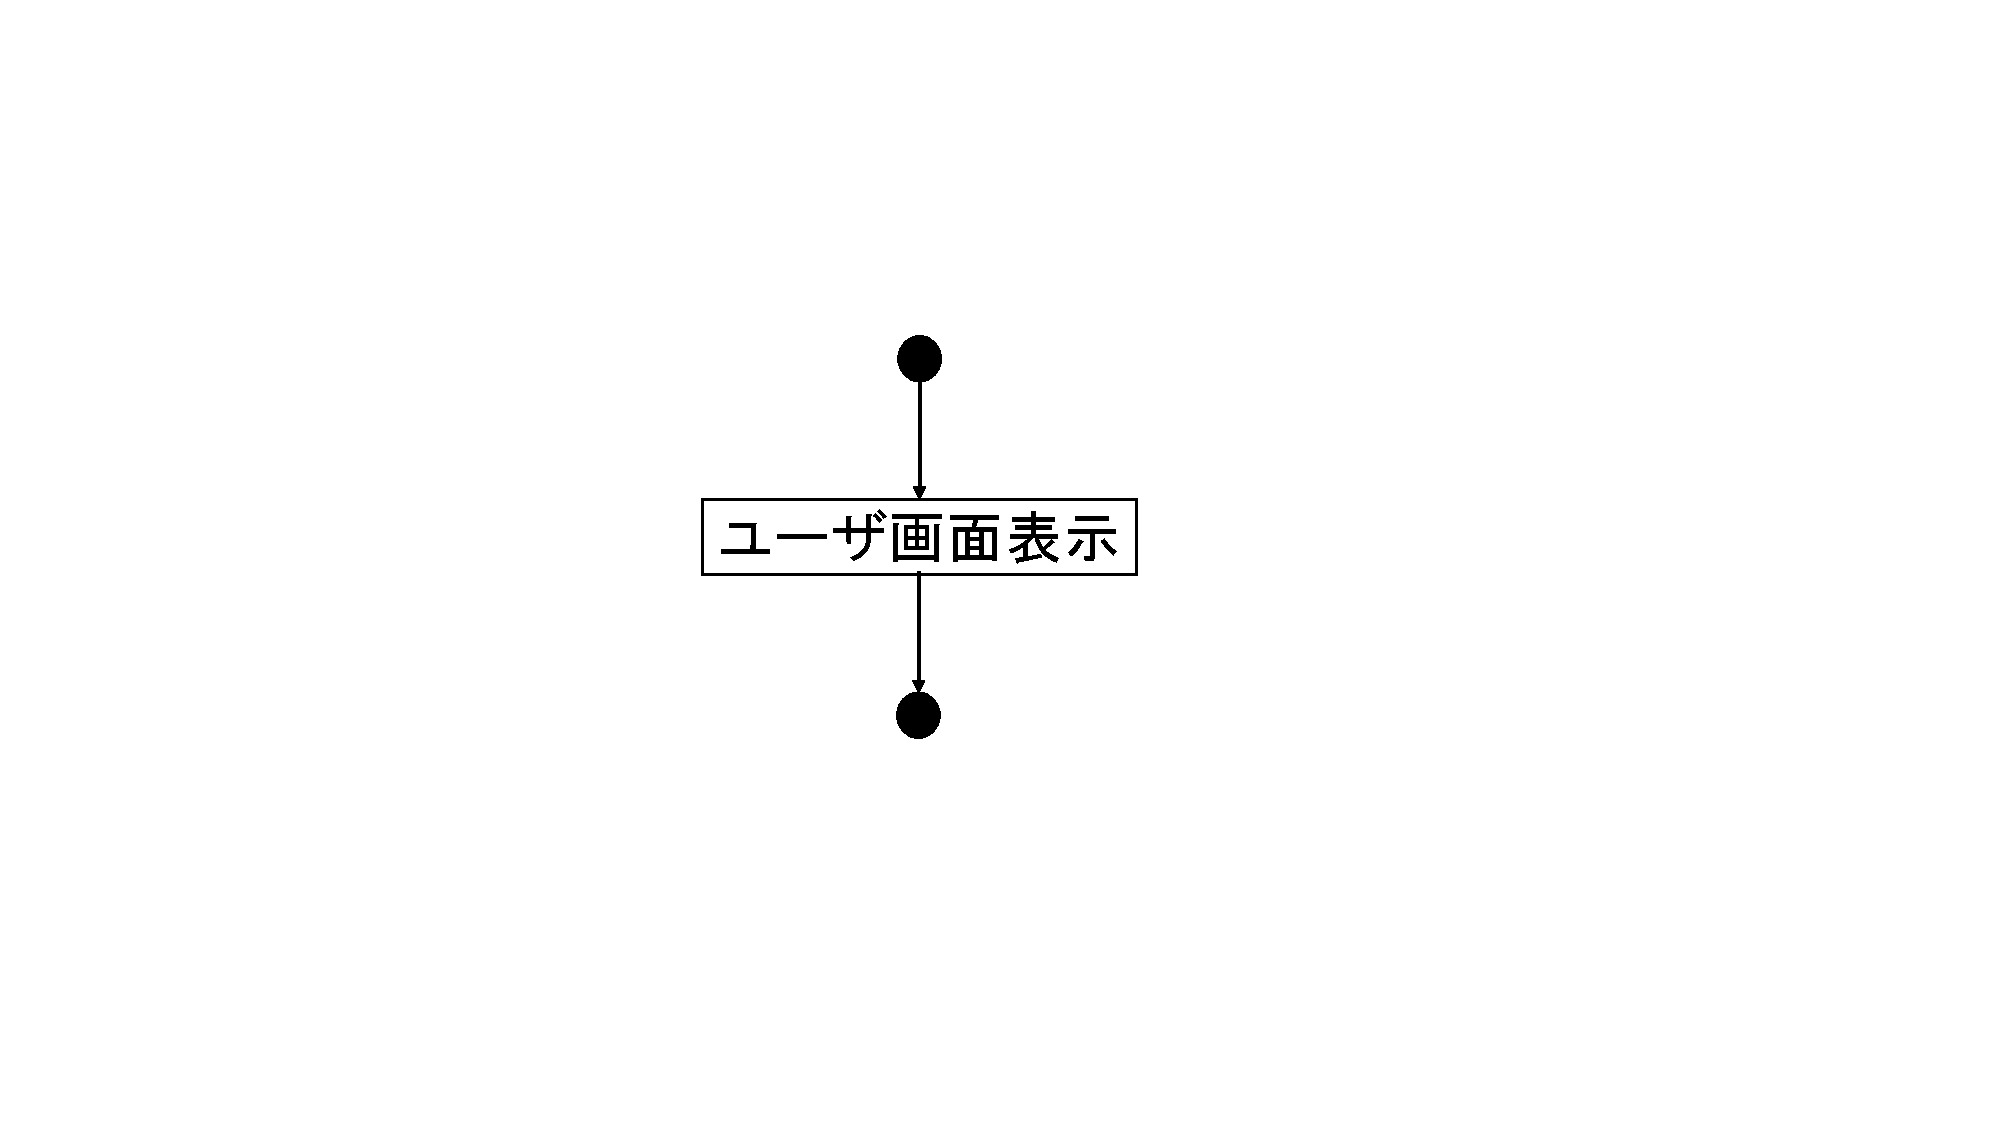
\includegraphics[width=13cm, bb=0 0 1000 540, clip]{./app_pic/app1-1.pdf}
	\caption{ユーザ画面表示モジュールの処理フロー}
	\label{fig;1-1}
	\end{center}
\end{figure}

\item dB値取得モジュール

図\ref{fig;1-2}に,dB値取得モジュールの処理フローを示す.

%図
\begin{figure}[H]
	\begin{center}
	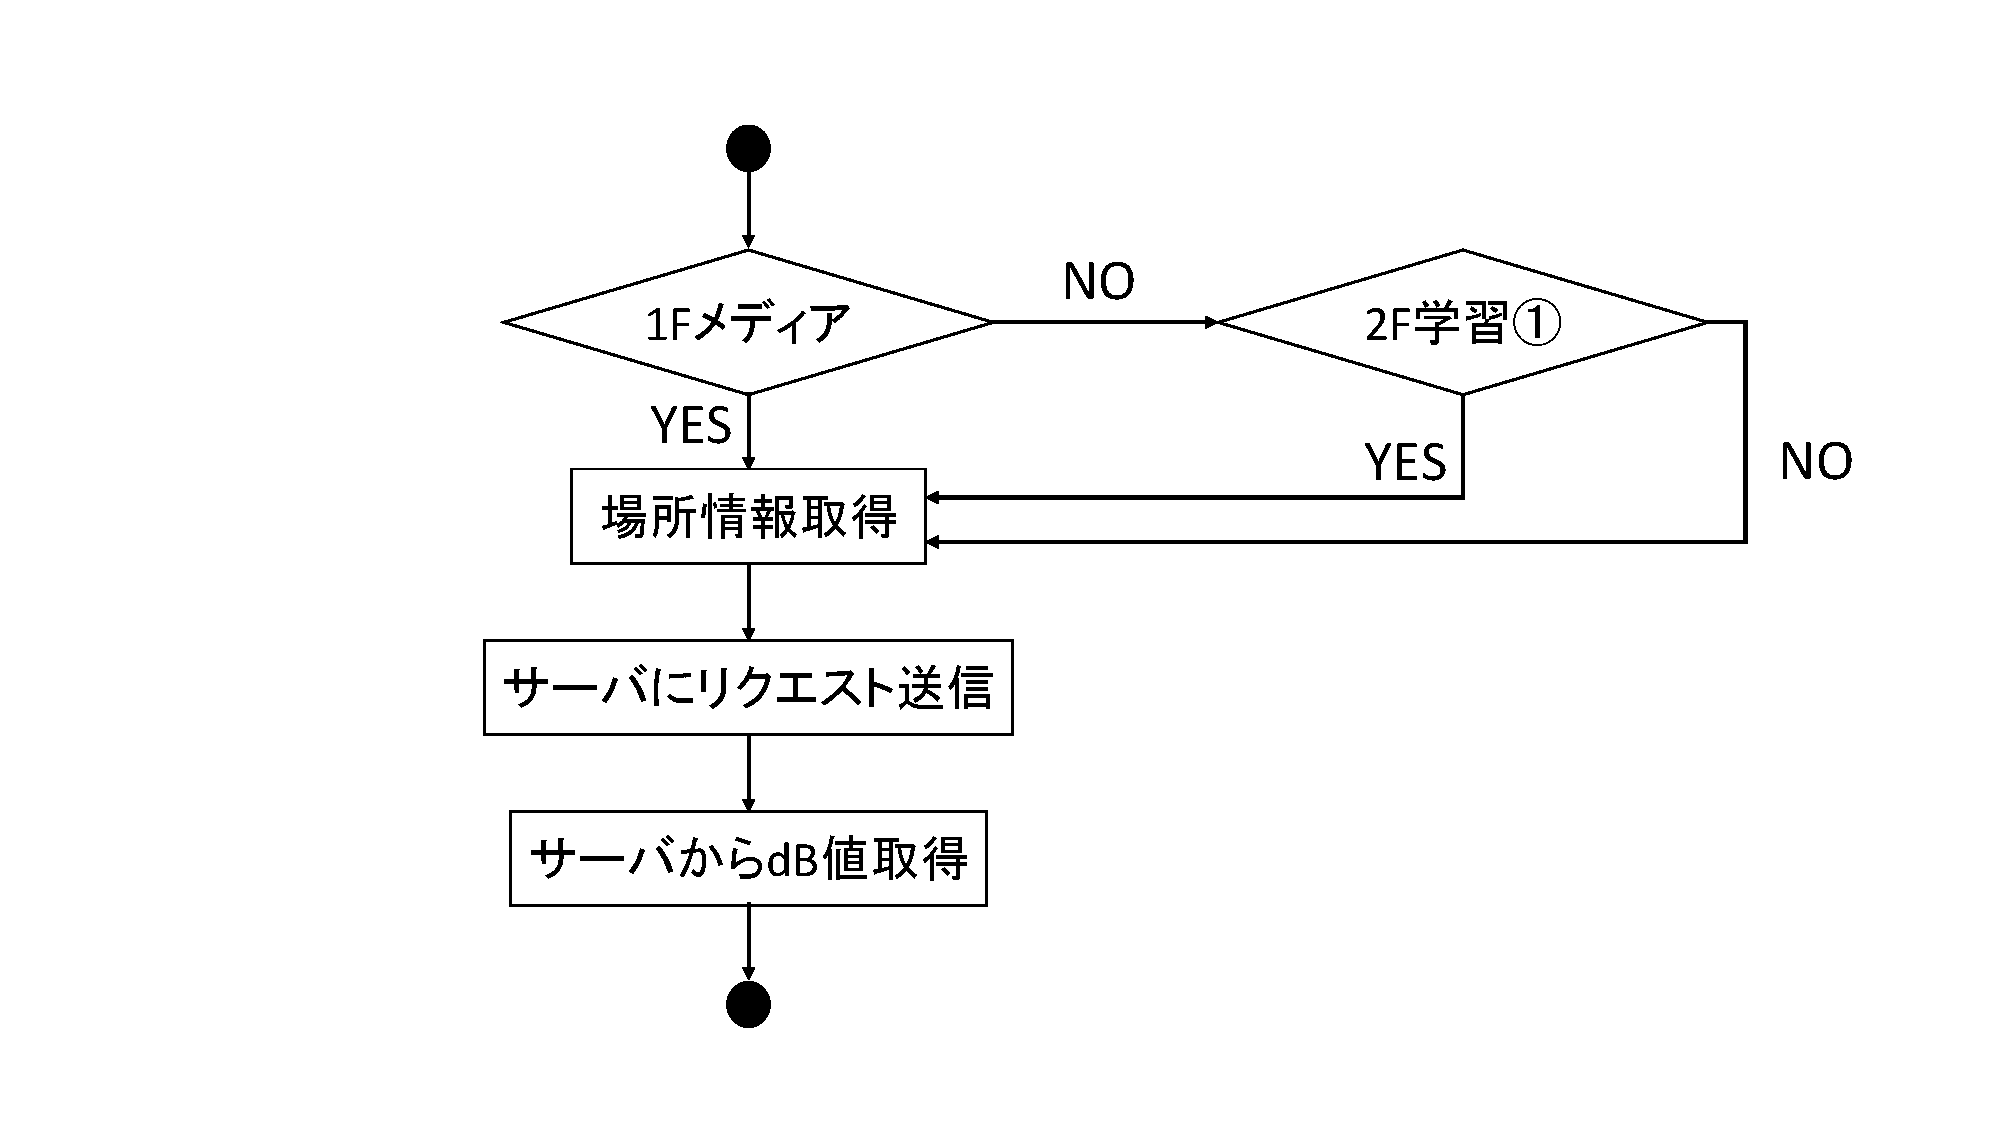
\includegraphics[width=15cm, bb=0 0 1000 540, clip]{./app_pic/app1-2.pdf}
	\caption{dB値取得モジュールの処理フロー}
	\label{fig;1-2}
	\end{center}
\end{figure}

\item データ計算モジュール

図\ref{fig;1-3}に,データ計算モジュールの処理フローを示す.

%図
\begin{figure}[H]
	\begin{center}
	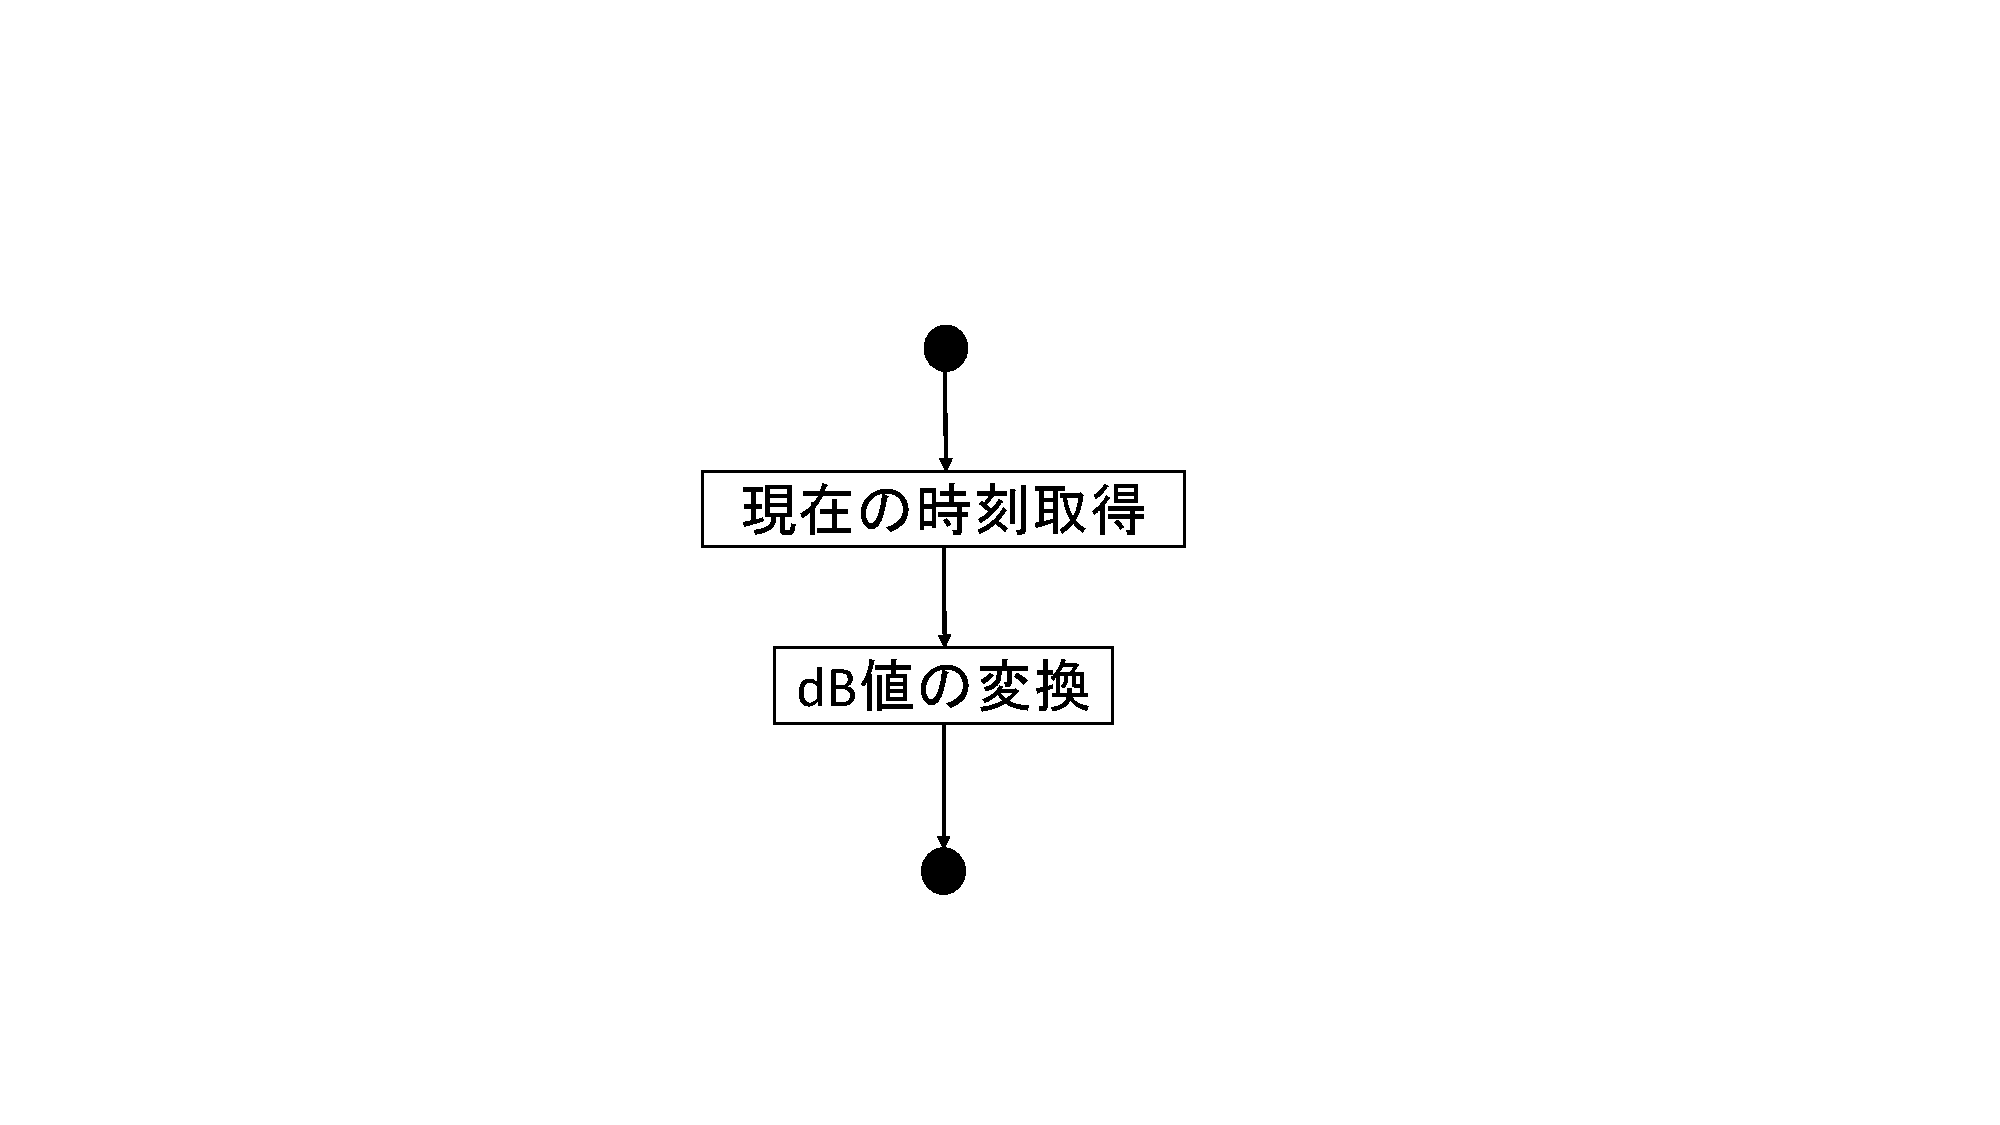
\includegraphics[width=15cm, bb=0 0 1000 540, clip]{./app_pic/app1-3.pdf}
	\caption{データ計算モジュールの処理フロー}
	\label{fig;1-3}
	\end{center}
\end{figure}

\item 画像取得モジュール

図\ref{fig;1-4}に,画像取得モジュールの処理フローを示す.

%図
\begin{figure}[H]
	\begin{center}
	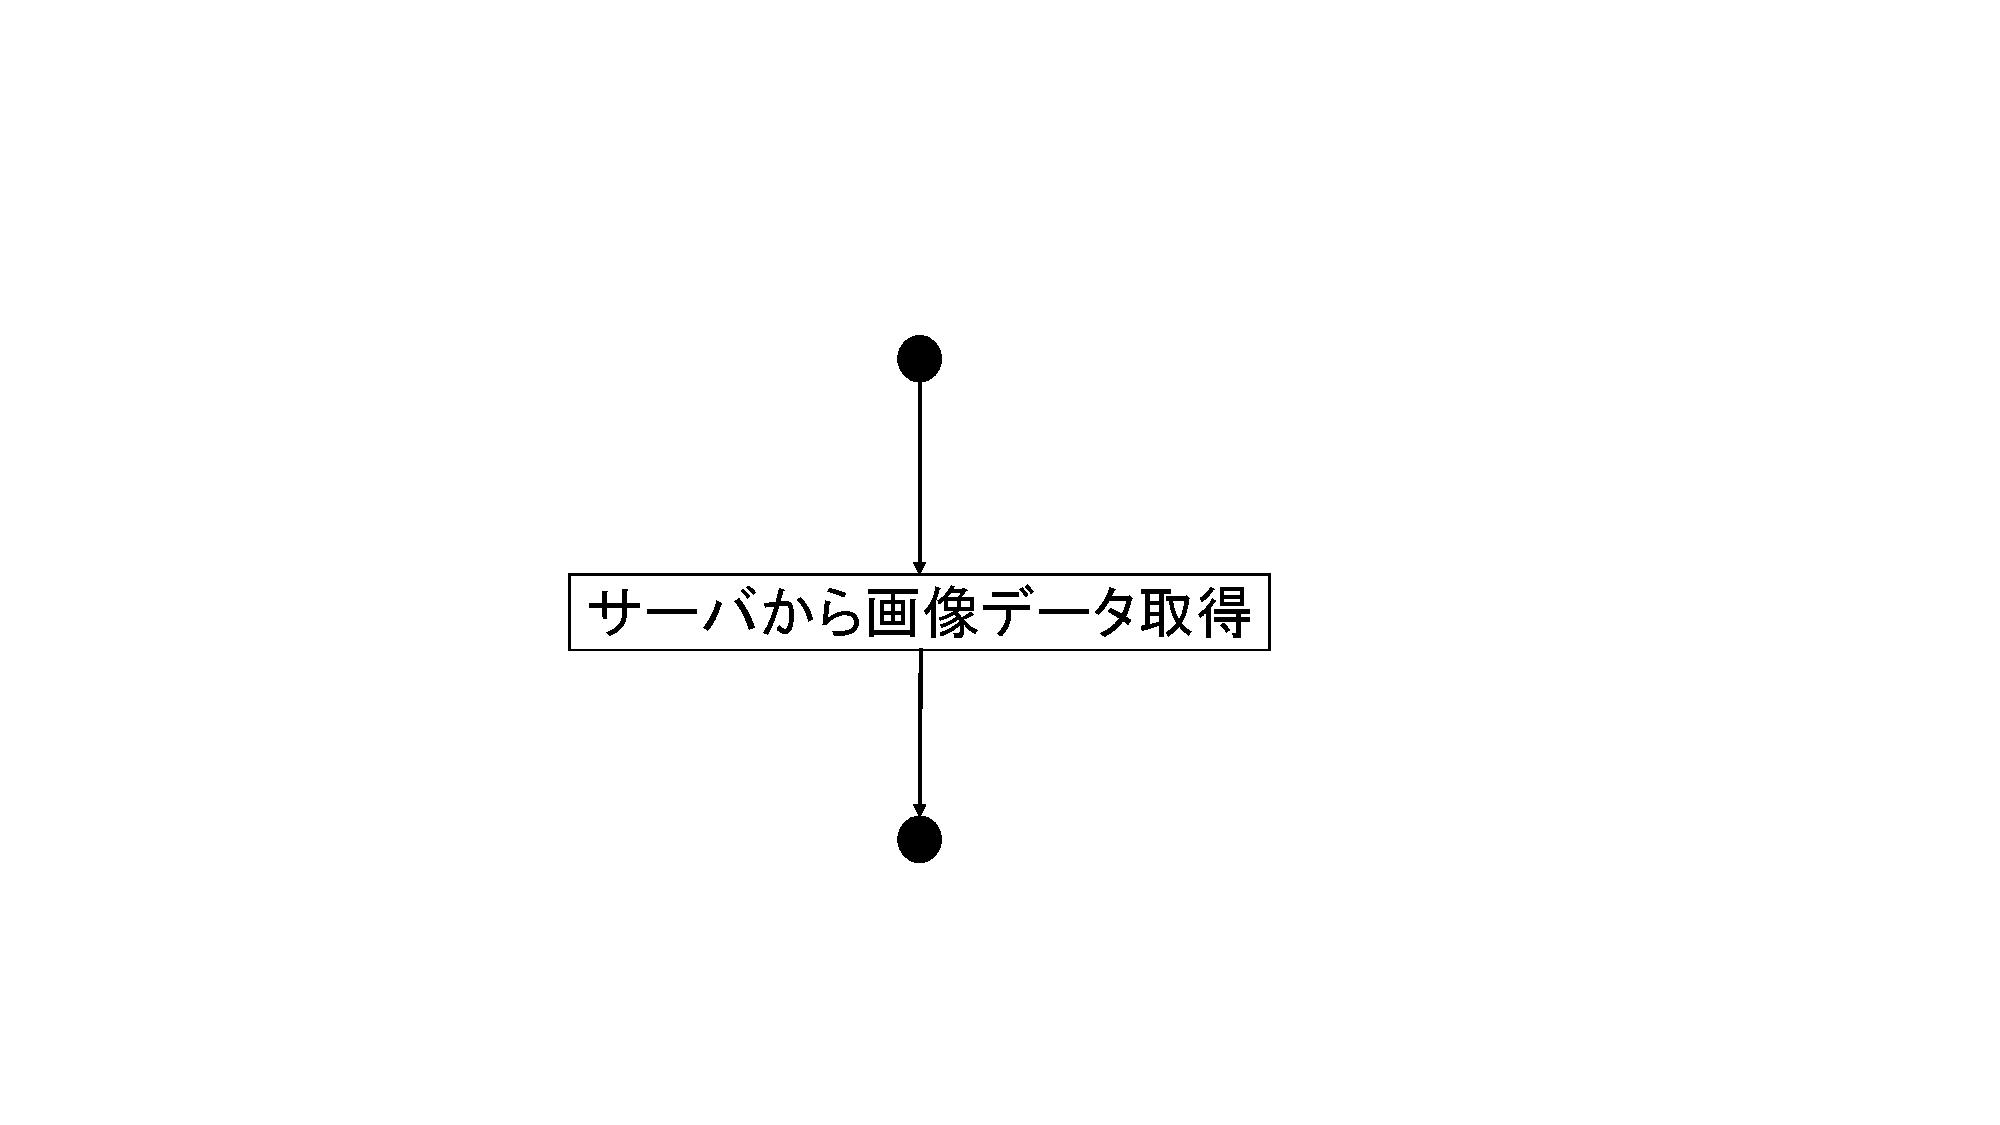
\includegraphics[width=15cm, bb=0 0 1000 540, clip]{./app_pic/app1-4.pdf}
	\caption{画像取得モジュールの処理フロー}
	\label{fig;1-4}
	\end{center}
\end{figure}

\item グラフ描画モジュール

図\ref{fig;1-5}に,グラフ描画モジュールの処理フローを示す.

%図
\begin{figure}[H]
	\begin{center}
	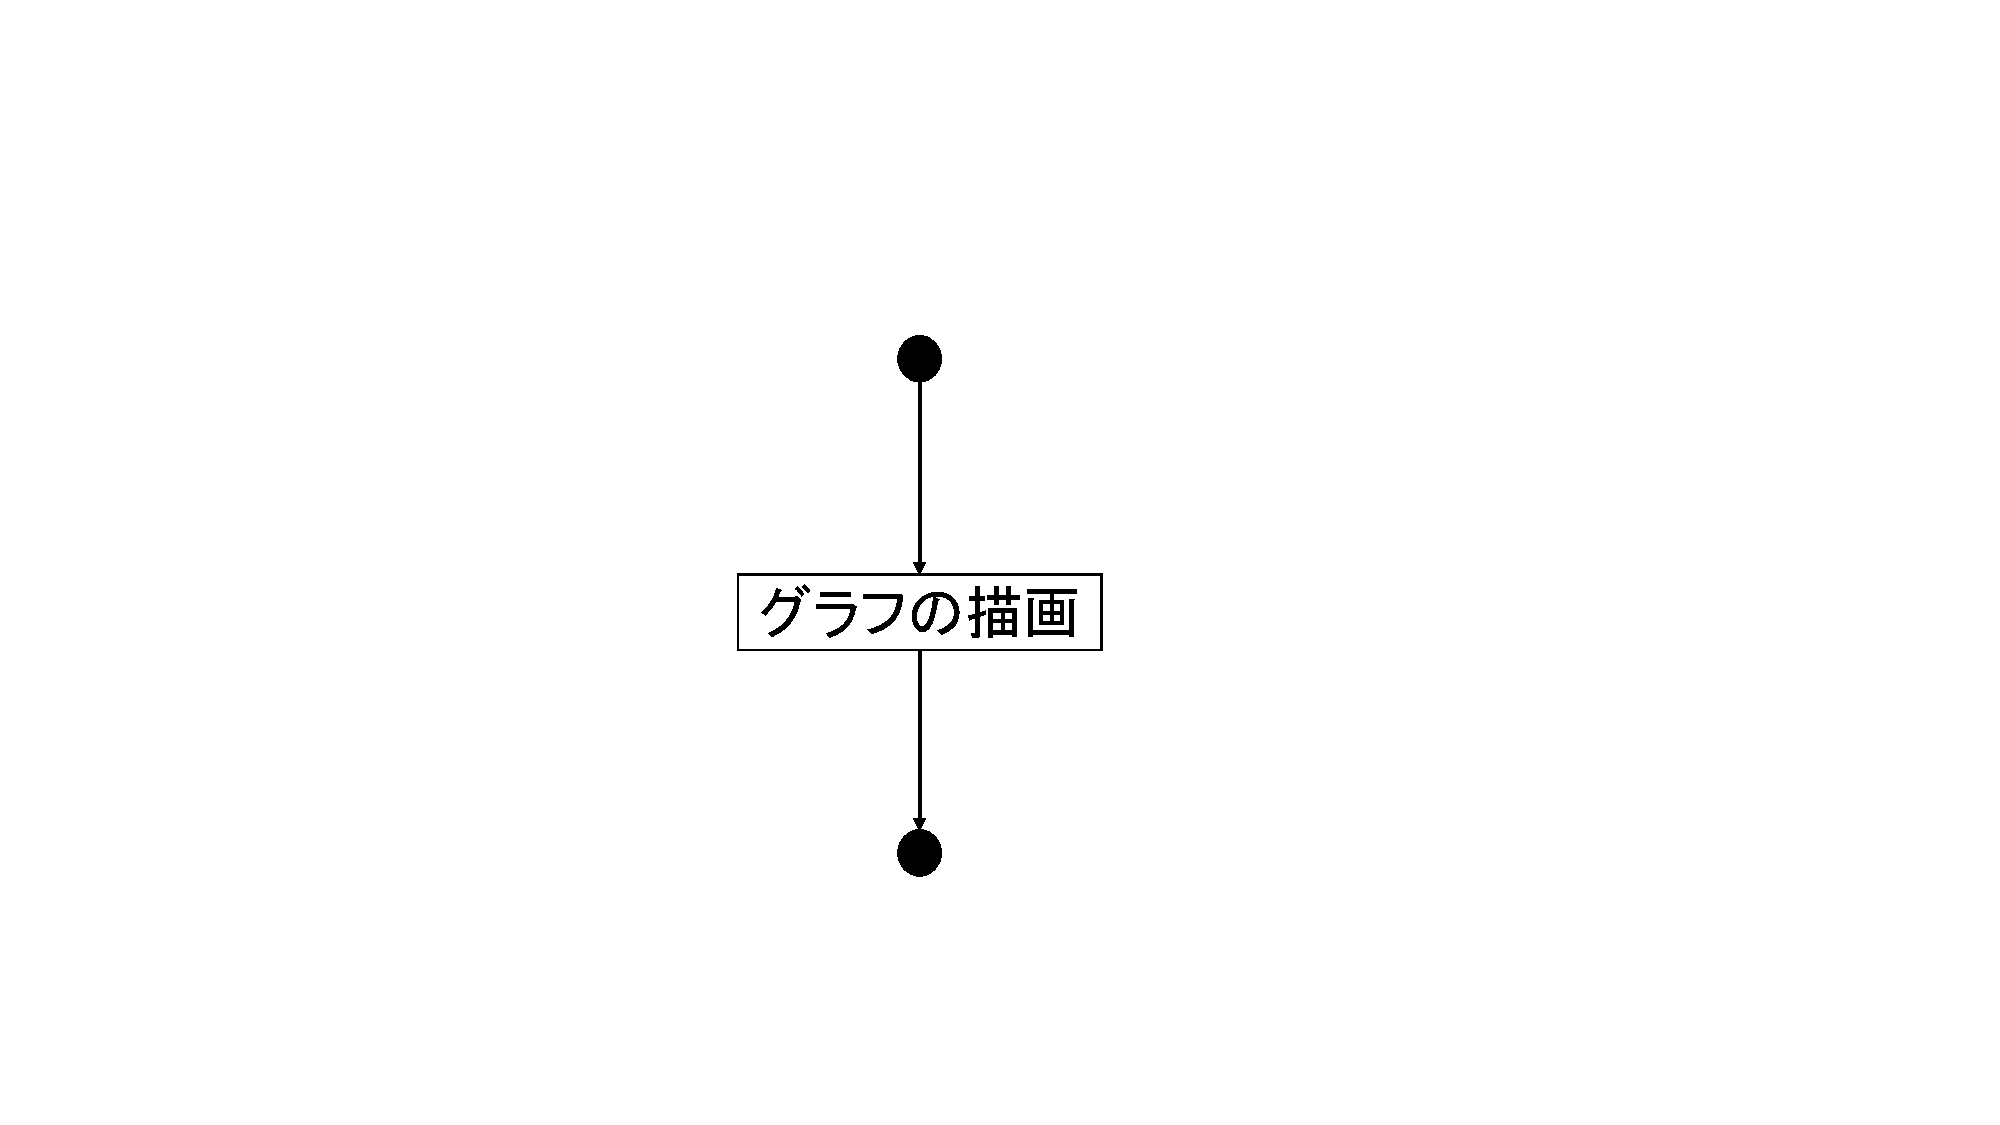
\includegraphics[width=15cm, bb=0 0 1000 540, clip]{./app_pic/app1-5.pdf}
	\caption{グラフ描画モジュールの処理フロー}
	\label{fig;1-5}
	\end{center}
\end{figure}

\item 騒音画面表示モジュール

図\ref{fig;1-6}に,騒音画面表示モジュールの処理フローを示す.

%図
\begin{figure}[H]
	\begin{center}
	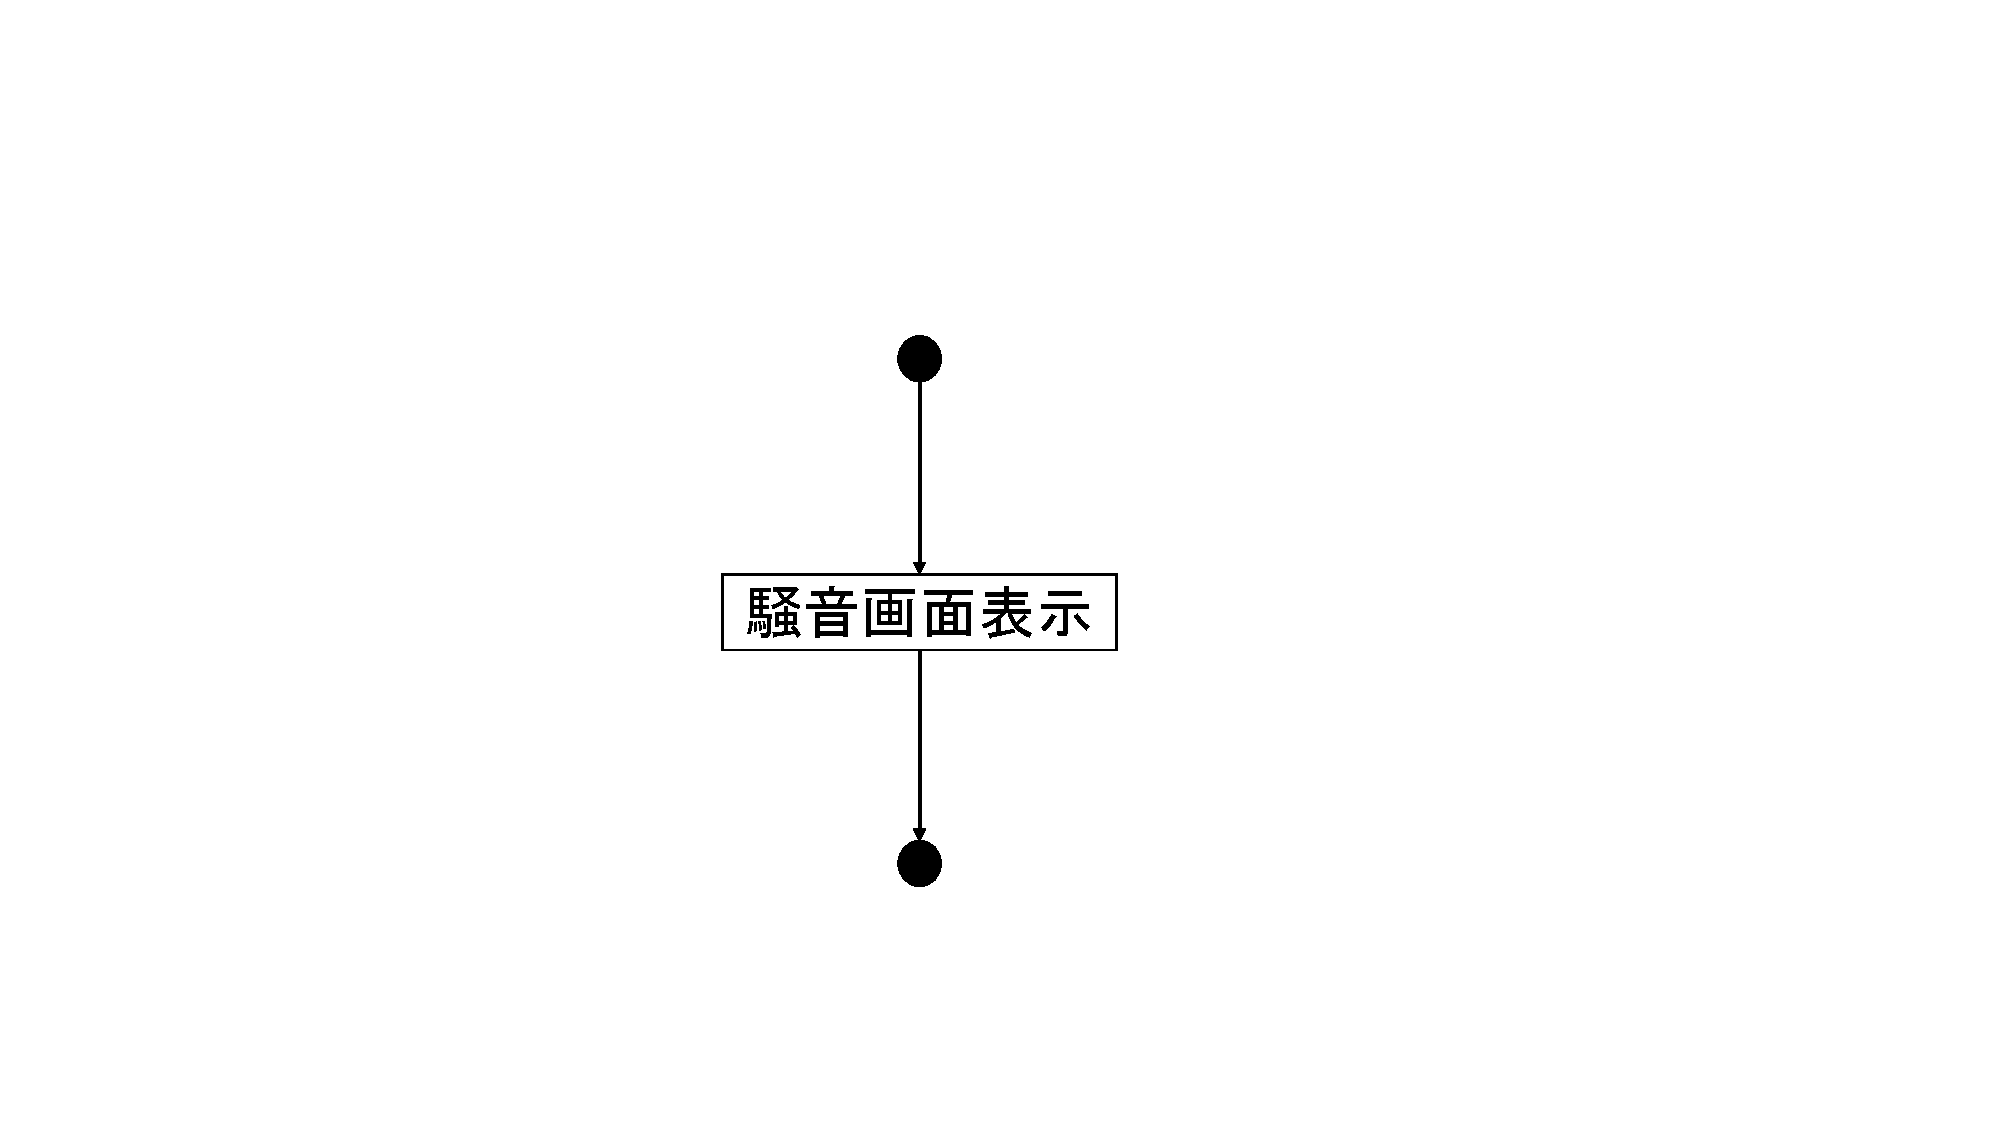
\includegraphics[width=15cm, bb=0 0 1000 540, clip]{./app_pic/app1-6.pdf}
	\caption{騒音画面表示モジュールの処理フロー}
	\label{fig;1-6}
	\end{center}
\end{figure}

\end{enumerate}
\subsubsection{システム管理に関するモジュール}
\begin{enumerate}
\renewcommand{\labelenumi}{(\arabic{enumi})}
\item 管理者画面表示モジュール

図\ref{fig;2-1}に,管理者画面表示モジュールの処理フローを示す.

%図
\begin{figure}[H]
	\begin{center}
	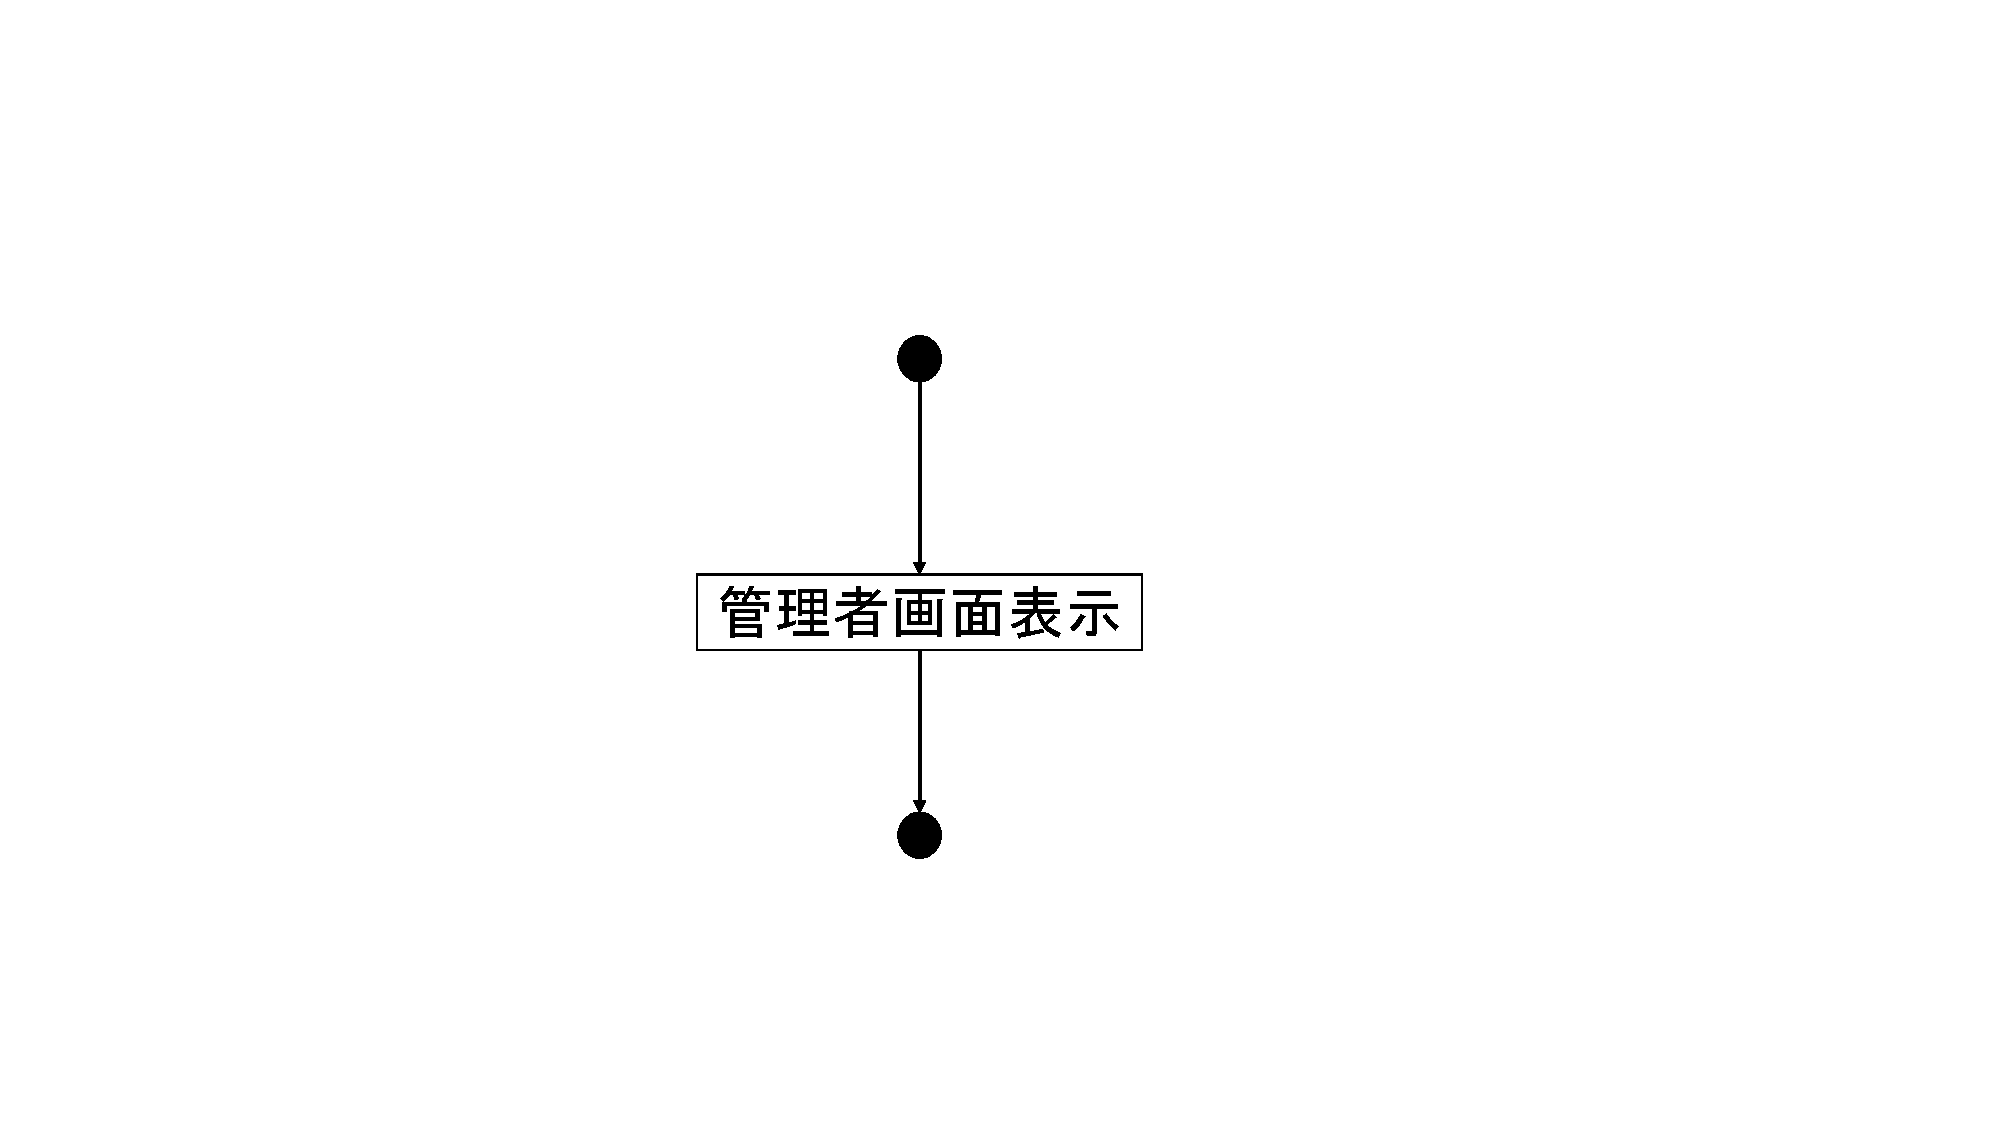
\includegraphics[width=15cm, bb=0 0 1000 540, clip]{./app_pic/app2-1.pdf}
	\caption{管理者画面表示モジュールの処理フロー}
	\label{fig;2-1}
	\end{center}
\end{figure}

\item ログイン画面表示モジュール

図\ref{fig;2-2}に,ログイン画面表示モジュールの処理フローを示す.

%図
\begin{figure}[H]
	\begin{center}
	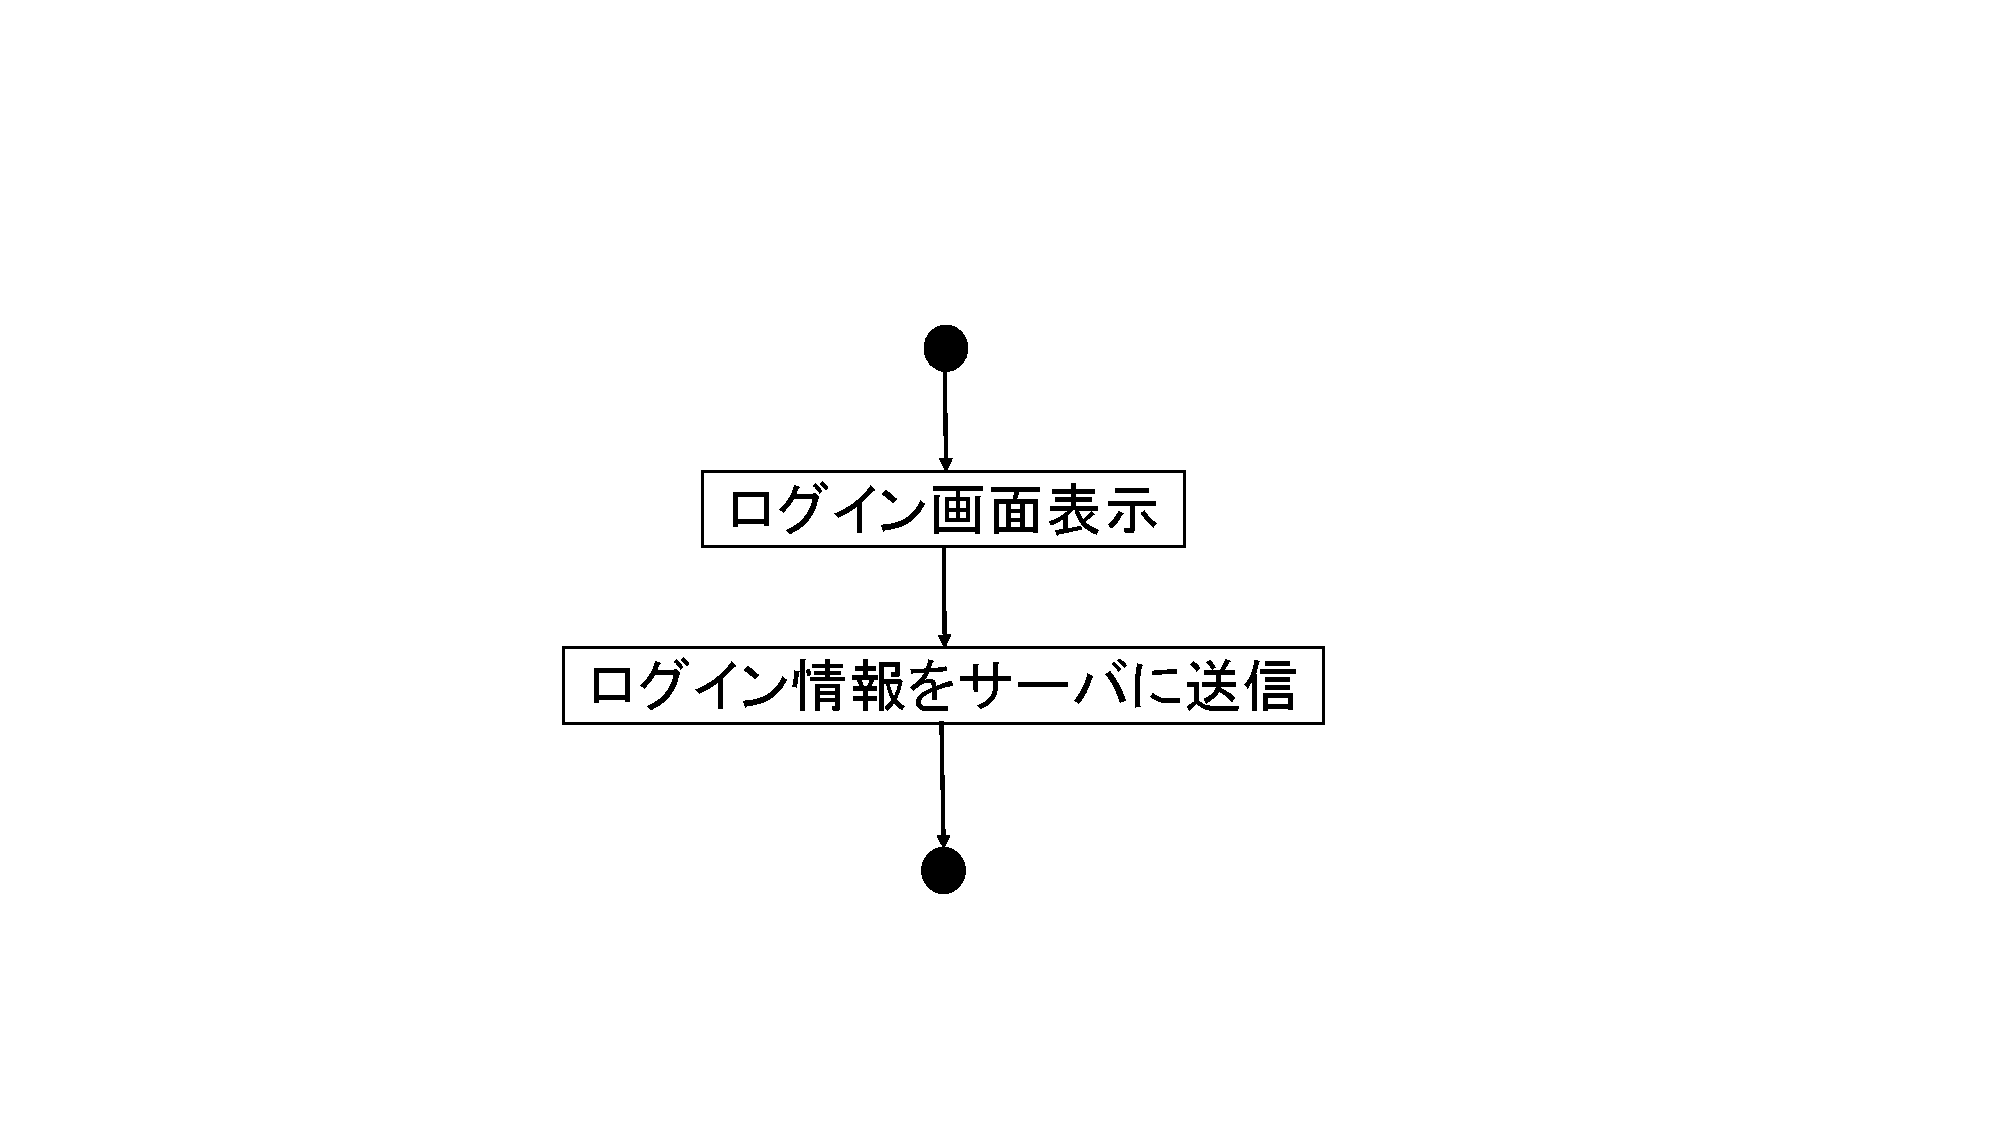
\includegraphics[width=15cm, bb=0 0 1000 540, clip]{./app_pic/app2-2.pdf}
	\caption{ログイン画面表示モジュールの処理フロー}
	\label{fig;2-2}
	\end{center}
\end{figure}

\item ログイン処理判定モジュール

図\ref{fig;2-3}に,ログイン処理判定モジュールの処理フローを示す.

\begin{figure}[H]
	\begin{center}
	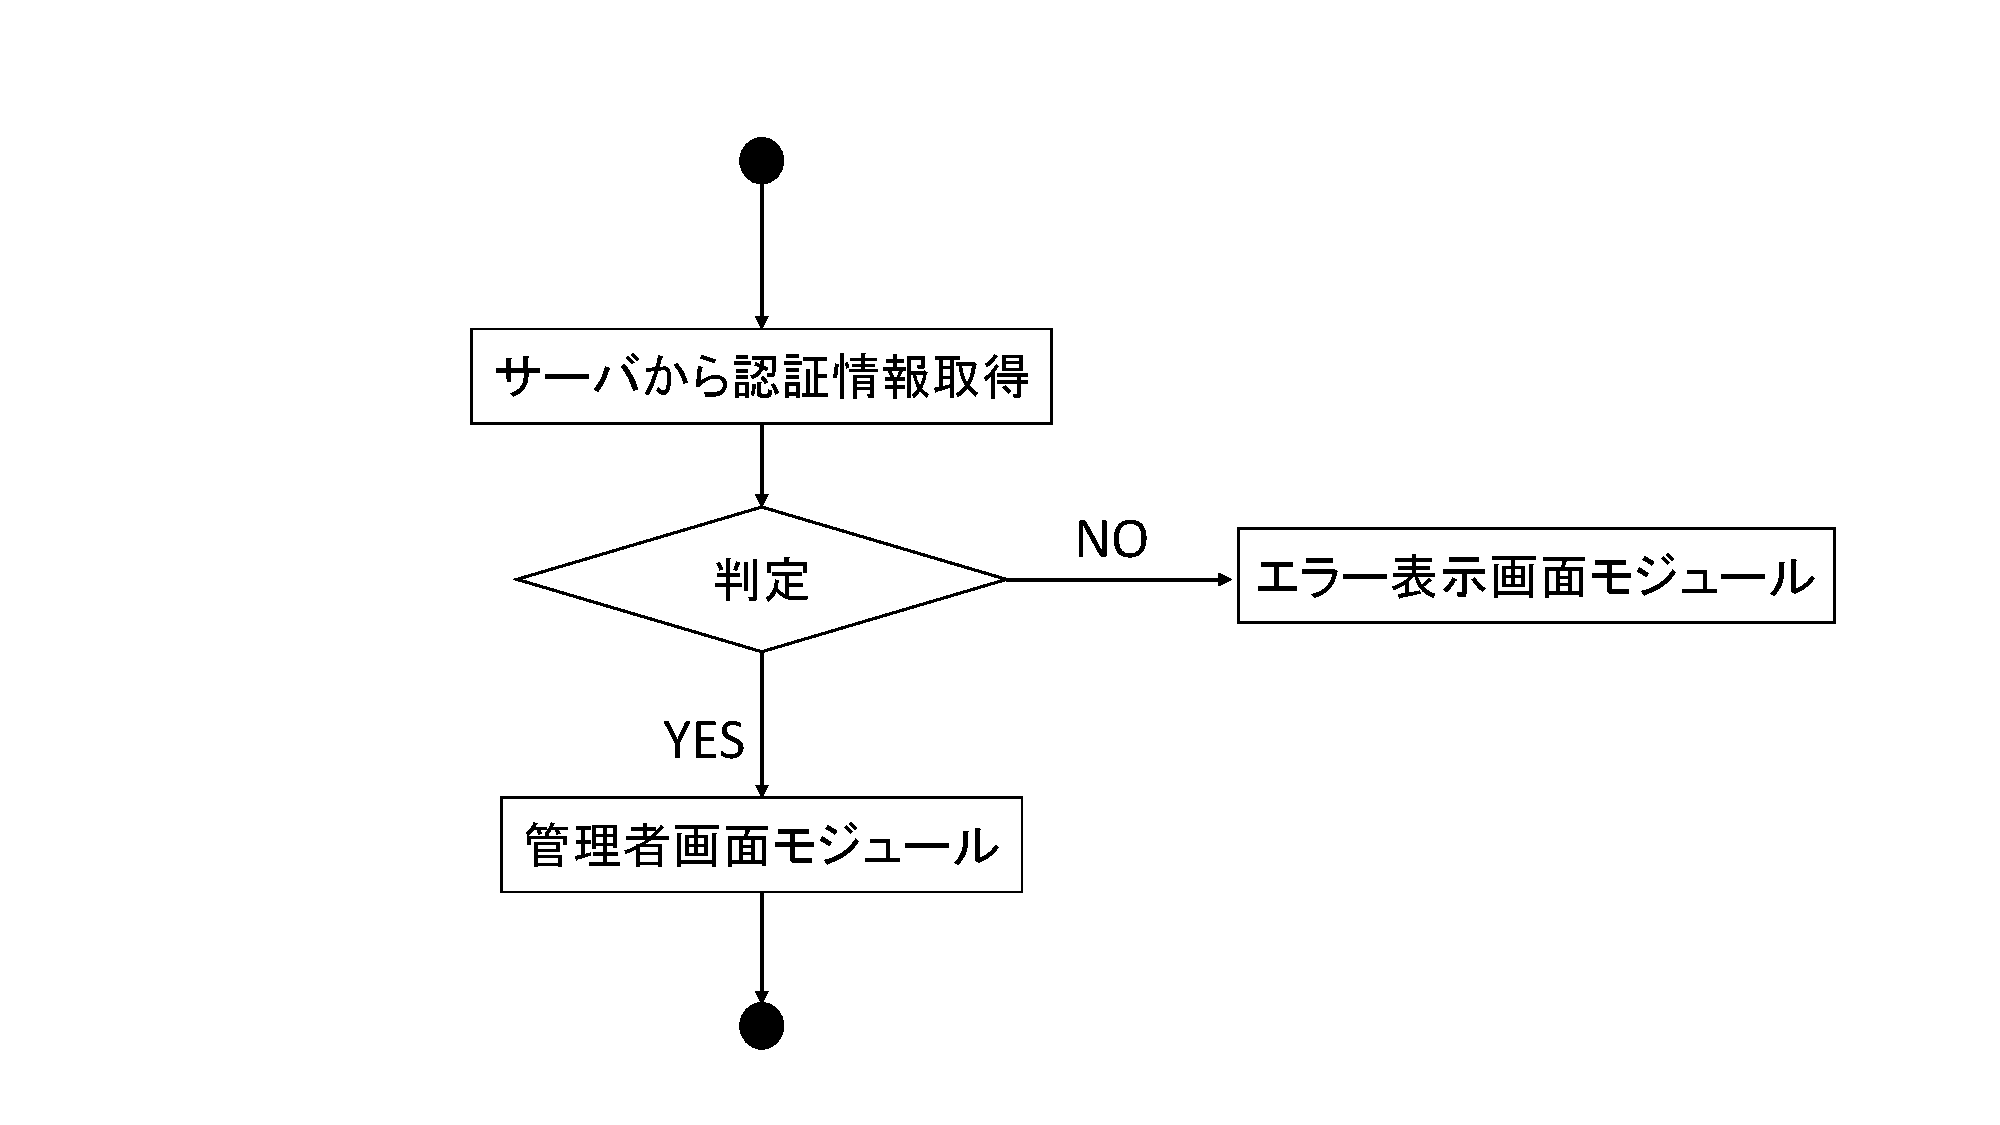
\includegraphics[width=15cm, bb=0 0 1000 540, clip]{./app_pic/app2-3.pdf}
	\caption{ログイン処理判定モジュールの処理フロー}
	\label{fig;2-3}
	\end{center}
\end{figure}

\item ログ情報表示モジュール

図\ref{fig;2-6}に,ログ情報表示モジュールの処理フローを示す.

%図
\begin{figure}[H]
	\begin{center}
	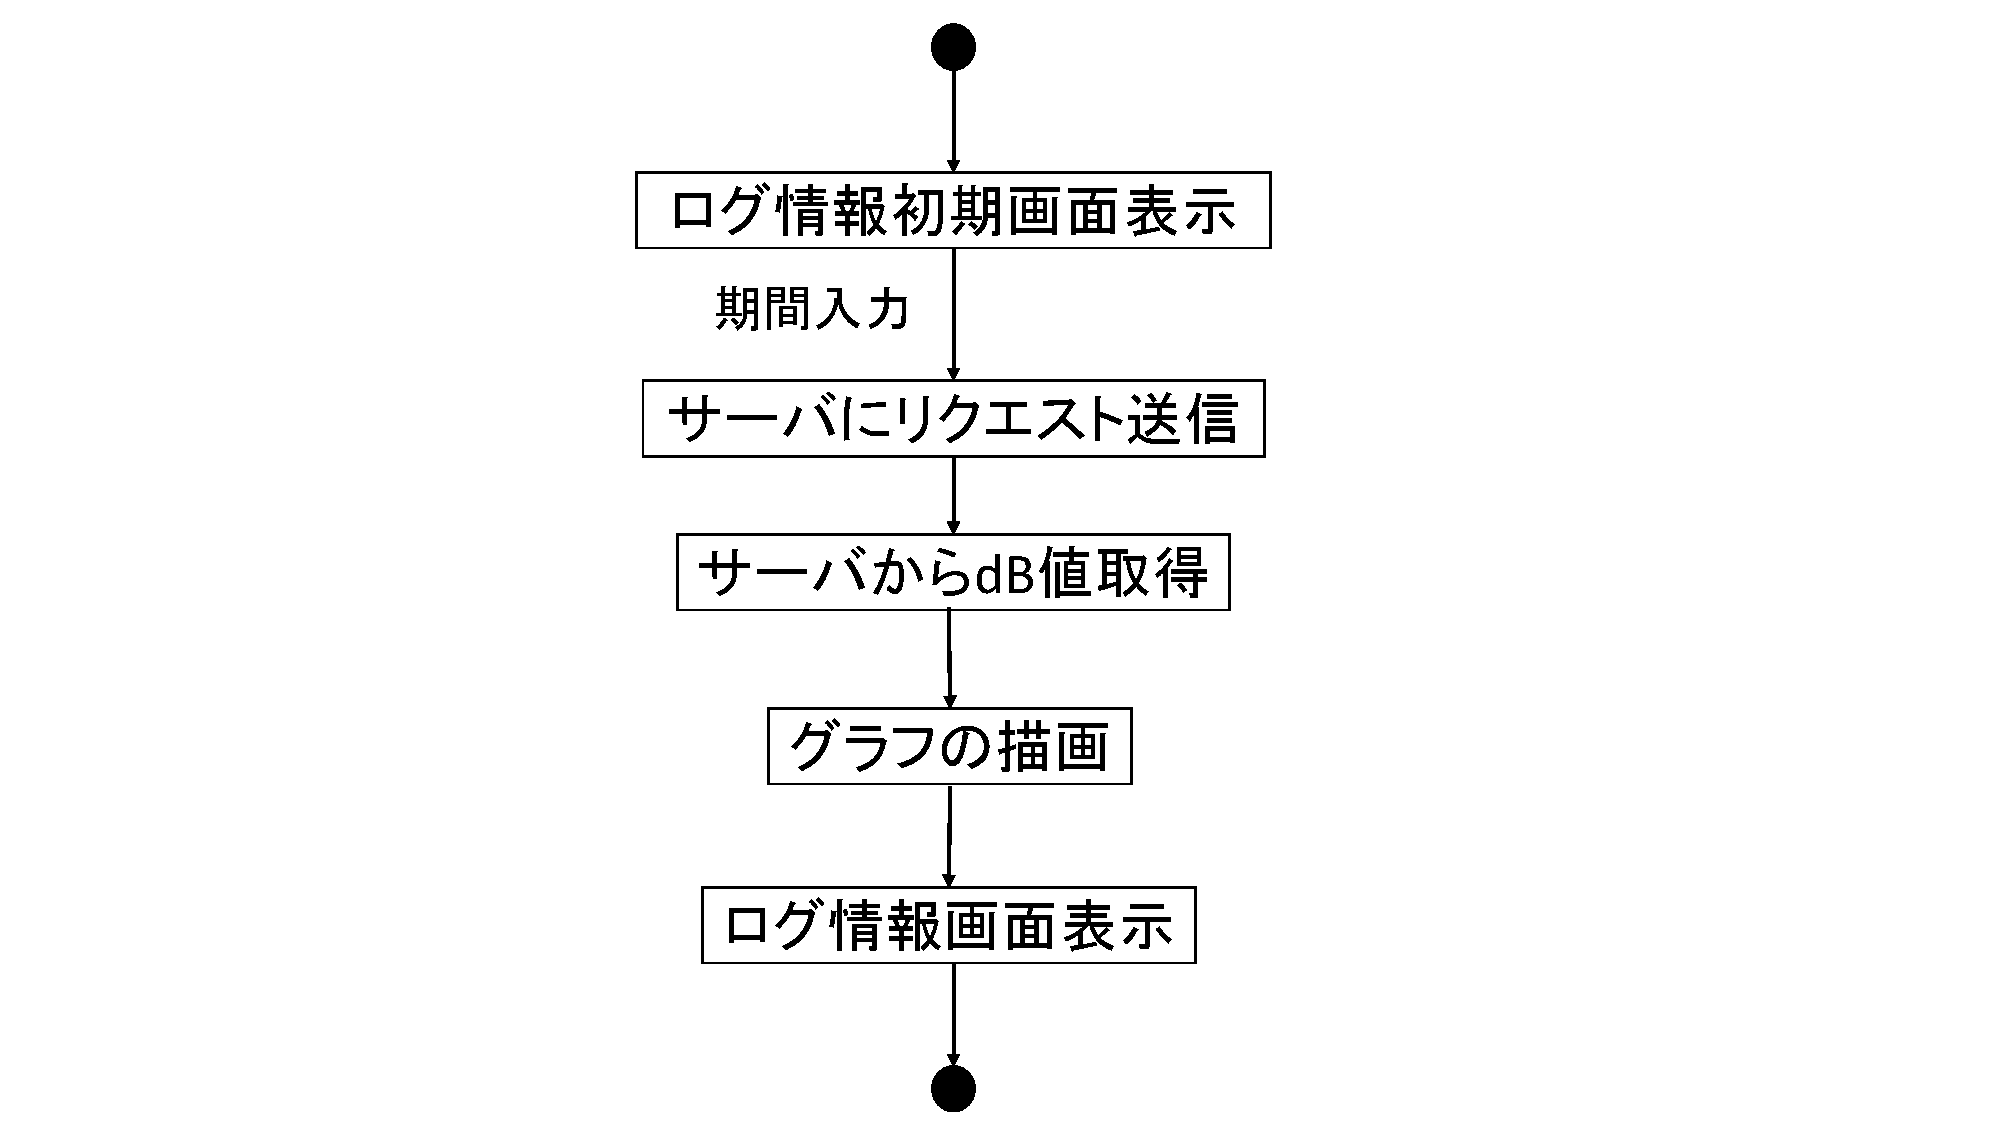
\includegraphics[width=15cm, bb=0 0 1000 540, clip]{./app_pic/app2-6.pdf}
	\caption{ログ情報表示モジュールの処理フロー}
	\label{fig;2-6}
	\end{center}
\end{figure}

\item エラー画面表示モジュール

図\ref{fig;2-4}に,エラー画面表示モジュールの処理フローを示す.

%図
\begin{figure}[H]
	\begin{center}
	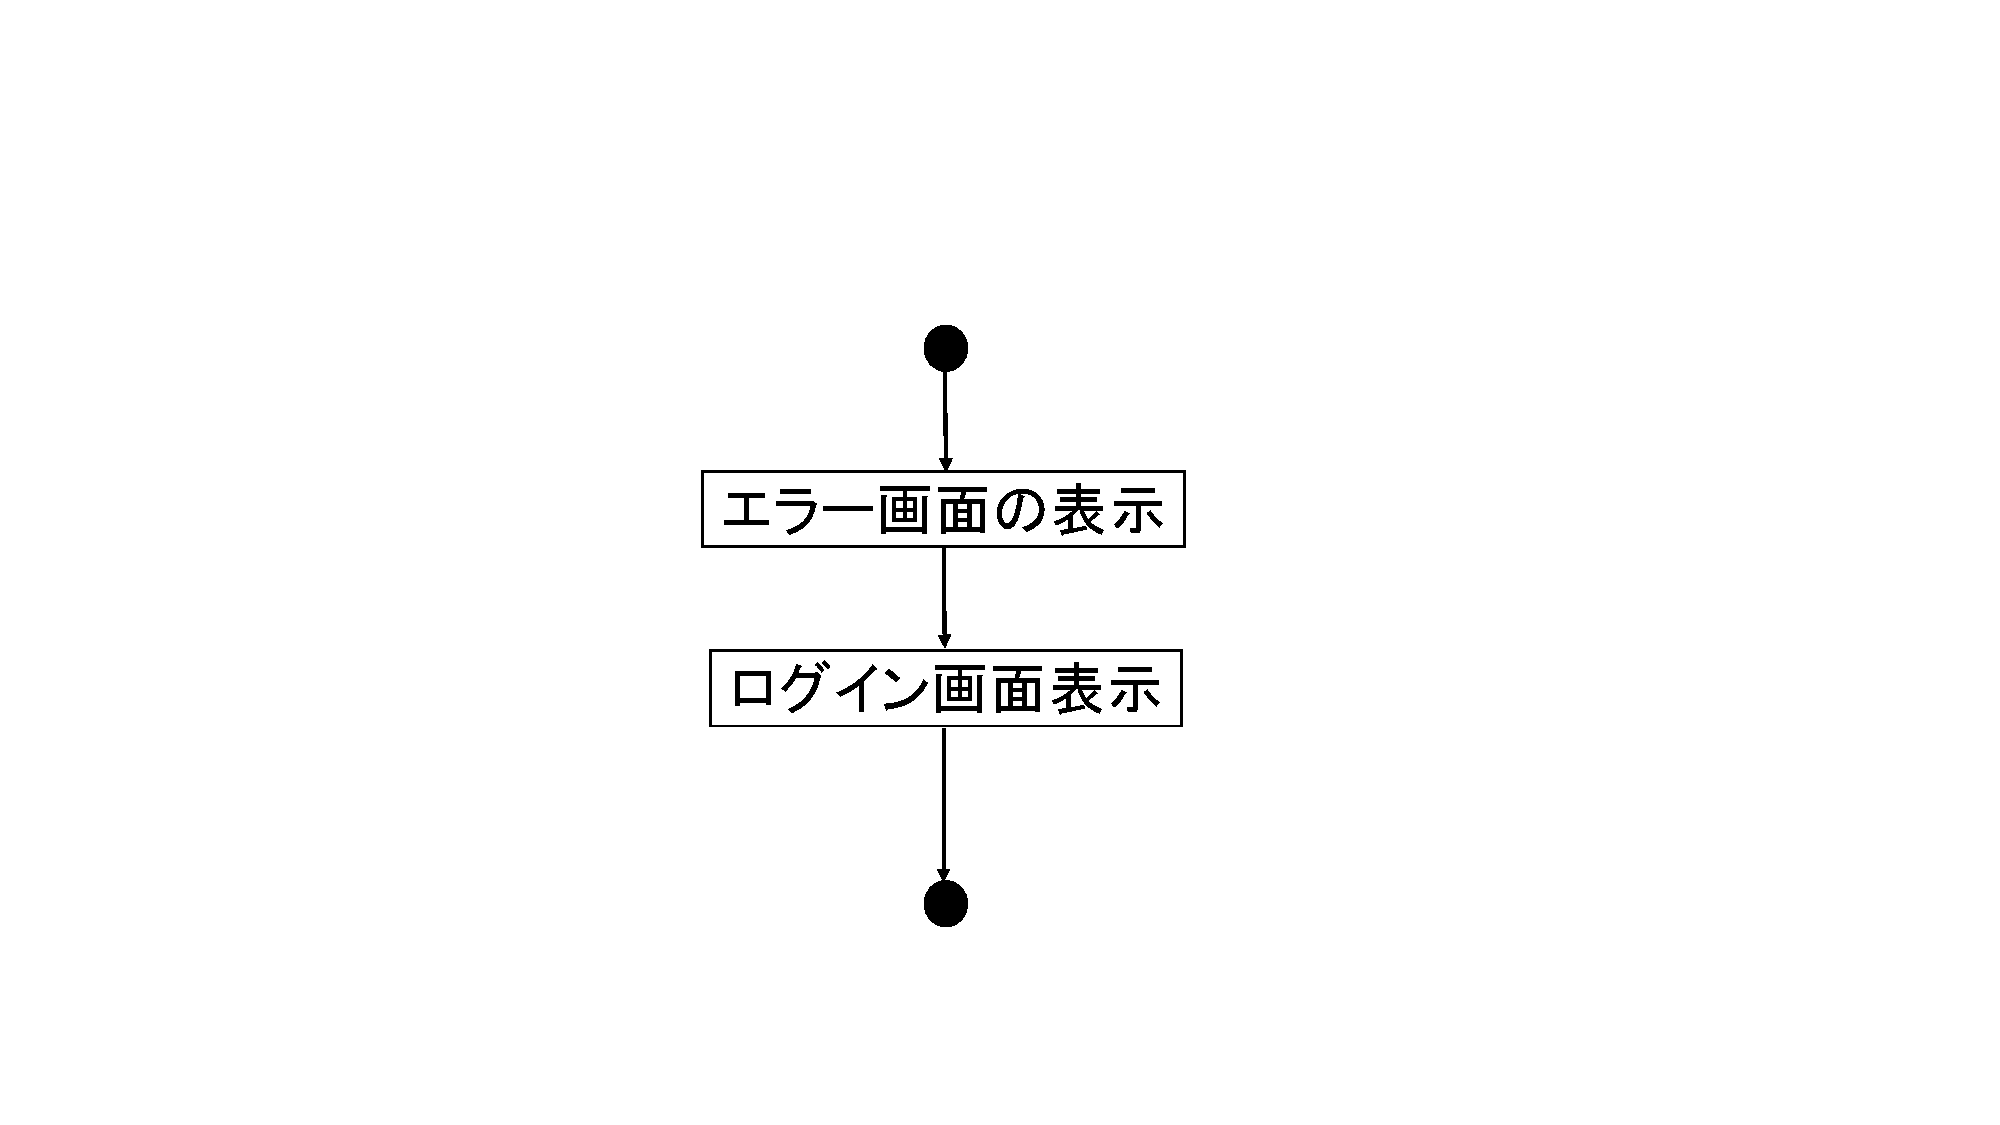
\includegraphics[width=15cm, bb=0 0 1000 540, clip]{./app_pic/app2-4.pdf}
	\caption{エラー画面表示モジュールの処理フロー}
	\label{fig;2-4}
	\end{center}
\end{figure}

\item 警告機能切替画面表示モジュール

図\ref{fig;2-5}に,警告機能切替画面表示モジュールの処理フローを示す.

%図
\begin{figure}[H]
	\begin{center}
	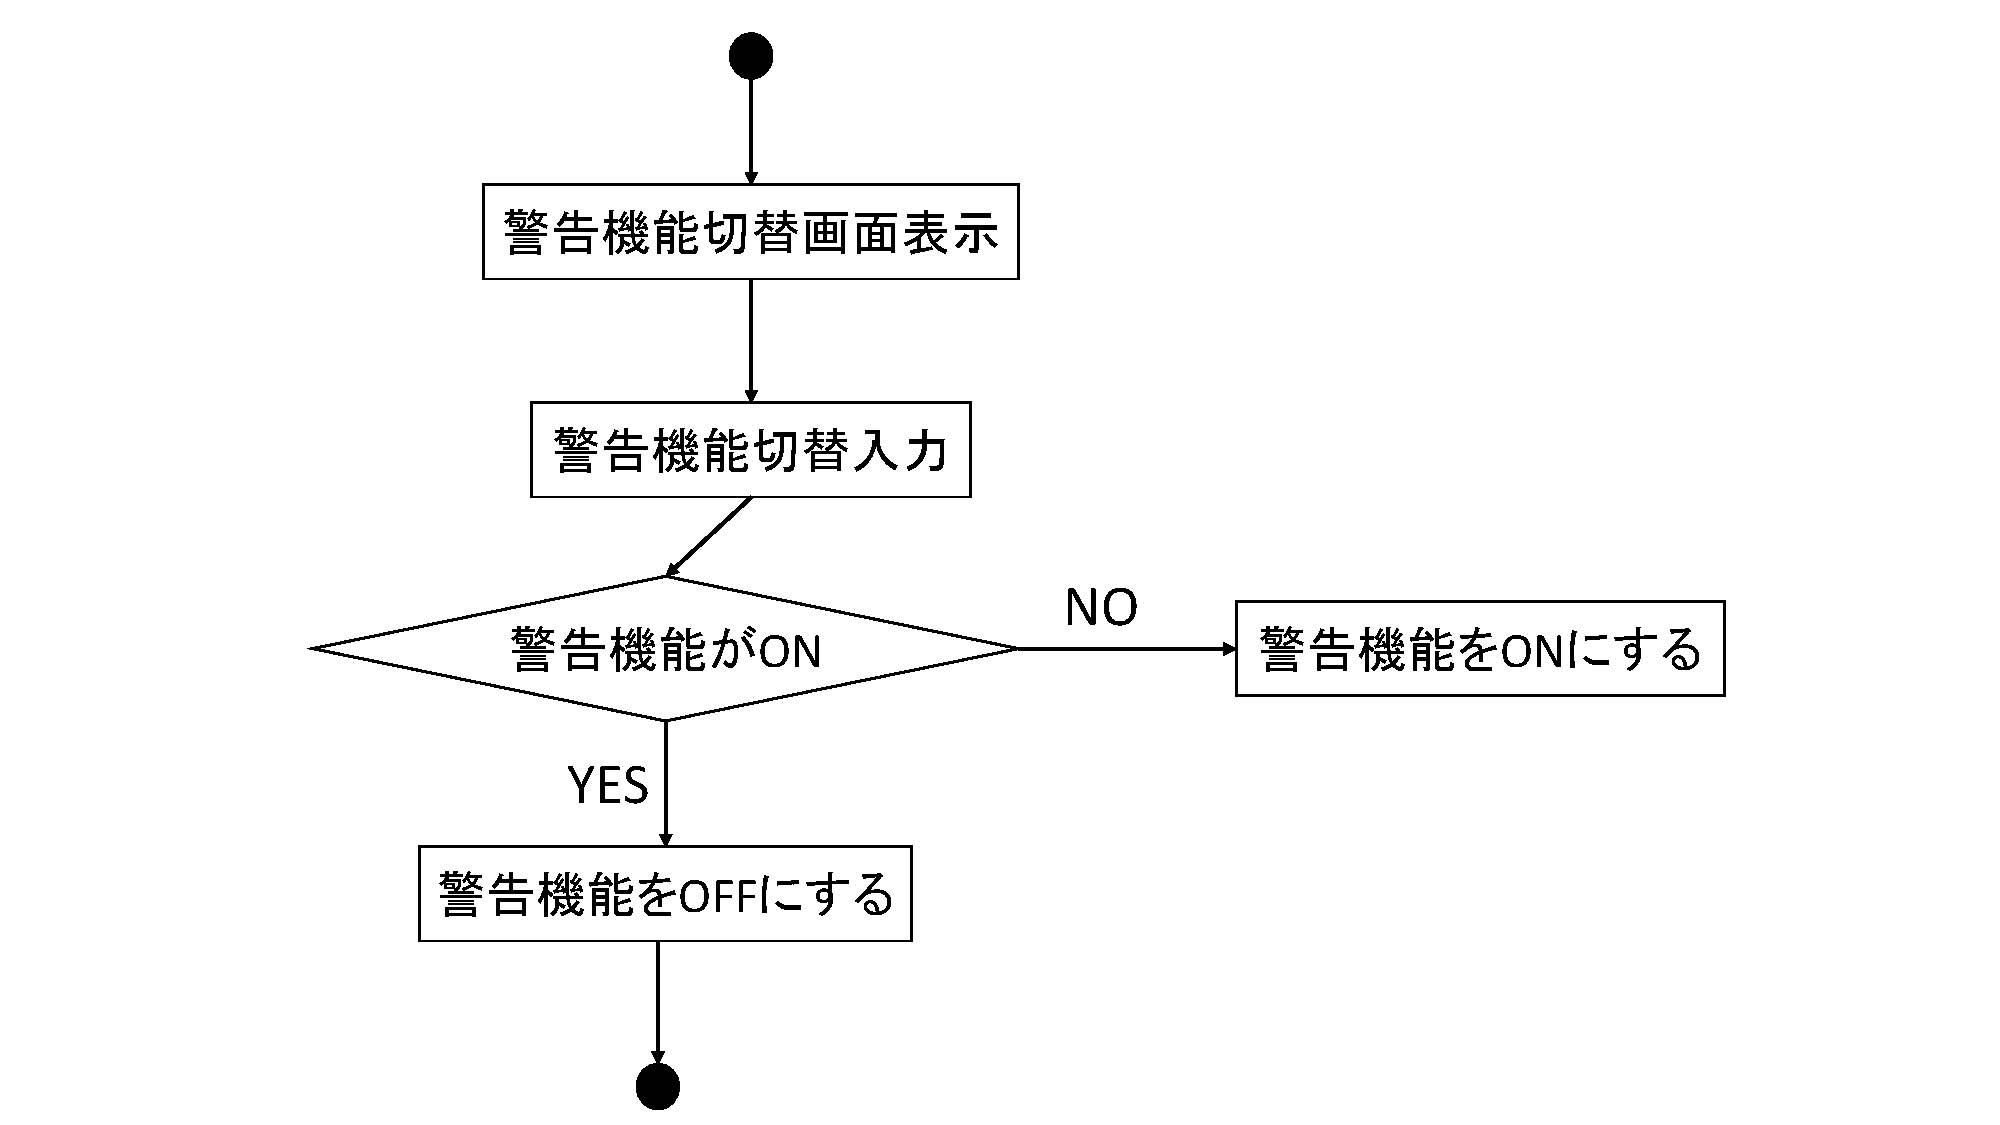
\includegraphics[width=15cm, bb=0 0 1000 540, clip]{./app_pic/app2-5.pdf}
	\caption{警告機能切替画面表示モジュールの処理フロー}
	\label{fig;2-5}
	\end{center}
\end{figure}



\end{enumerate}
\subsubsection{騒音情報取得,警告音発信に関するメソッド}

\subsection{モジュール(メソッド)インタフェース}
\subsubsection{騒音情報表示に関するモジュール}
\begin{enumerate}
\renewcommand{\labelenumi}{(\arabic{enumi})}
\item ユーザ画面表示モジュール

\begin{itemize}
\item モジュール名:
\item 引数:
\item 戻り値:
\end{itemize}


\item dB値取得モジュール
\begin{itemize}
\item モジュール名:
\item 引数:
\item 戻り値:
\end{itemize}
\item データ計算モジュール
\begin{itemize}
\item 
\item 
\item
\end{itemize}
\item 画像取得モジュール
\begin{itemize}
\item 
\item 
\item
\end{itemize}
\item グラフ描画モジュール
\begin{itemize}
\item 
\item 
\item
\end{itemize}
\item 騒音画面表示モジュール
\begin{itemize}
\item 
\item 
\item
\end{itemize}
\item データ成型モジュール
\begin{itemize}
\item 
\item 
\item
\end{itemize}
\item アプリからの入力受付モジュール
\begin{itemize}
\item 
\item 
\item
\end{itemize}
\end{enumerate}
\subsubsection{システム管理に関するモジュール}
\begin{enumerate}
\renewcommand{\labelenumi}{(\arabic{enumi})}
\item 管理者画面表示モジュール
\begin{itemize}
\item 
\item 
\item
\end{itemize}
\item ログイン画面表示モジュール
\begin{itemize}
\item 
\item 
\item
\end{itemize}
\item ログイン処理判定モジュール
\begin{itemize}
\item 
\item 
\item
\end{itemize}
\item ログ情報表示モジュール
\begin{itemize}
\item 
\item 
\item
\end{itemize}
\item エラー画面表示モジュール
\begin{itemize}
\item 
\item 
\item
\end{itemize}
\item 警告機能切替画面表示モジュール
\begin{itemize}
\item 
\item 
\item
\end{itemize}
\item 警告音判定モジュール
\begin{itemize}
\item 
\item 
\item
\end{itemize}
\item 認証モジュール
\begin{itemize}
\item 
\item 
\item
\end{itemize}
\item 警告機能制御モジュール
\begin{itemize}
\item 
\item 
\item
\end{itemize}
\end{enumerate}
\subsubsection{騒音情報取得,警告音発信に関するメソッド}
\begin{enumerate}
\renewcommand{\labelenumi}{(\arabic{enumi})}
\item 電圧取得・増幅メソッド
\begin{itemize}
	\item メソッド名 : get\_voltage
	\item 引数 : なし
	\item 戻り値 : なし\\
\end{itemize}
	\begin{itemize}
	\item メソッド名 : amplification\_voltage
	\item 引数 : 浮動小数点数(電圧)
	\item 戻り値 : なし\\
	\end{itemize}
\item 電圧/dB値変換メソッド
	\begin{itemize}
	\item メソッド名 : convertion\_voltage\_to\_decibel
	\item 引数 : 浮動小数点数(電圧)
	\item 戻り値 : なし\\
	\end{itemize}
\item dB値平均算出メソッド
	\begin{itemize}
	\item メソッド名 : calc\_avg\_val\_for\_1\_minute
	\item 引数 : 浮動小数点数(dB値)
	\item 戻り値 : なし\\
	\end{itemize}
\item 騒音情報作成メソッド
	\begin{itemize}
	\item メソッド名 : create\_sysdata
	\item 引数 : 浮動小数点数(1分間の平均dB値)
	\item 戻り値 : なし \\
	\end{itemize}
\item 騒音情報送信メソッド
	\begin{itemize}
	\item メソッド名 : send\_data\_to\_server
	\item 引数 : なし
	\item 戻り値 : なし \\
	\end{itemize}
\item 警告命令受信メソッド
	\begin{itemize}
	\item メソッド名 : reseive\_warning\_or\_stop\_instruction
	\item 引数 : 整数(1 : 警告命令,0 : 警告停止命令)
	\item 戻り値 : なし \\
	\end{itemize}
\end{enumerate}
\end{document}
